%This work is licensed by the author, Isaakidis Marios, under the Creative Commons Attribution 3.0 Unported License, in memory of Aaron Swartz. To view a copy of this license, visit http://creativecommons.org/licenses/by/3.0/ or send a letter to Creative Commons, 444 Castro Street, Suite 900, Mountain View, California, 94041, USA.

\documentclass[12pt,a4paper,oneside]{article}
\usepackage{graphicx}
\usepackage{tikz}
\usepackage{hyperref}
\usepackage{nomencl}
\usepackage{pdfpages}
\usepackage{listings}

\lstdefinelanguage{diff}{
  morecomment=[f][\color{blue}]{@@},     % group identifier
  morecomment=[f][\color{red}]-,         % deleted lines 
  morecomment=[f][\color{green}]+,       % added lines
  morecomment=[f][\color{magenta}]{---}, % Diff header lines (must appear after +,-)
  morecomment=[f][\color{magenta}]{+++},
  breaklines=true,breakindent=0pt,breakatwhitespace=true,
  postbreak=\raisebox{0ex}[0ex][0ex]{\ensuremath{\color{black}\hookrightarrow\space}},
  basicstyle=\ttfamily\small
}

\makenomenclature

\begin{document}

% TODO Add CUT template titlepage

%Insert titlepage
\pagenumbering{roman}
\pdfbookmark[0]{Title}{title}
\begin{titlepage}

\begin{center}

\newcommand{\HRule}{\rule{\linewidth}{0.5mm}}

% Upper part of the page   
\textsc{\large FINAL THESIS PROGRESS REPORT}\\[1.5cm]


% Title
\HRule \\[0.5cm]
{ \LARGE \bfseries {\huge ServalDHT} \\[0.2cm] A Decentralized Service Resolution\\[0.2cm]Service for the Serval Architecture}\\[0.5cm]

\HRule \\[1cm]

{\LARGE \bf
Isaakidis Marios\\
}
misaakidis@yahoo.gr

\vfill

% Bottom of the page
{\large
The research and implementation ideas described in this report are developed under the advisement of Dr. Sirivianos Michael.}
\end{center}
 ~\\[1.5cm]
\begin{flushright}

\includegraphics[width=0.25\textwidth]{./cut-logo-2}\\ 
{\large
December 2012 \\
Cyprus University of Technology
}
\end{flushright}



\end{titlepage}
\phantomsection
\pdfbookmark[0]{Copyright}{cc}
\clearpage\null\vfill
\thispagestyle{empty}
\begin{center}
\setcounter{page}{3}
\pdfbookmark[0]{Copyright}{cc}
Copyright \copyright \href{https://creativecommons.org/licenses/by/3.0/}{CC-BY 3.0} 2012--\the\year\ Isaakidis Marios\\[0.5cm]
Permission is granted to copy and distribute this document under the terms of the Creative Commons Attribution 3.0 Unported License\ldots.
\end{center}

The approval of the diploma thesis by the Department of Electrical Engineering, Computer Engineering and Informatics of the Cyprus University of Technology does not necessarily imply acceptance of the views of the author on behalf of the Department.

\clearpage


%%%%%%%%%%%%%%%%%%%%%%%%%%%%%%%%%%%%%%%%%%%%%%%%%%%%%%%%%%%%%%%%%%%%
\newpage
\thispagestyle{empty}
\pdfbookmark[0]{Acknowledgements}{acks}
{\Large \bf \noindent Acknowledgements}
\\Here go the acknowledgements


%%%%%%%%%%%%%%%%%%%%%%%%%%%%%%%%%%%%%%%%%%%%%%%%%%%%%%%%%%%%%%%%%%%%
\newpage
\thispagestyle{empty}
\pdfbookmark[0]{ABSTRACT}{abstract}
{\Large \bf \noindent Abstract} \\[0.13cm]

\noindent The concept of the Internet has radically changed since its first onset, around half a century ago; millions of multi-homed users, often moving across networks, are asking for data and services offered by multiple servers, which can be replicated and situated in various geographical locations.
Yet only a few modifications managed to consolidate and provide the framework for communicating in the largest computer network.

This situation is leading to erratic band-aids where network administrators and developers overload the existing network abstractions or resort to middleware, in order to provide the supplementary functionality needed by a network where services and data become first-class citizens.

In this thesis we are introducing the approach of Service-Aware Networking, a consolidation of Service-Centric abstractions and the Software Defined Networking (SDN)\nomenclature{SDN}{Software Defined Networking} paradigm.

Starting with an explanation of the principles behind Service-Centric networking, we are focusing on the Serval architecture along with its functional prototype.
Results of benchmarks are presented juxtaposed to the measurements of the unmodified TCP/IP stack.

Finally we are suggesting that Software Defined Networking could benefit from Serval's service-level data plane and enable services running in – possibly distributed – datacenters to automatically, and according to the rights they have been granted, manipulate virtual networks to better utilize the underlying network infrastructure, conforming to their dynamic needs.\\[0.1cm]

\noindent The project is Open Source and can be found at\\ 
\noindent \href{https://github.com/misaakidis/ServalDHT}{https://github.com/misaakidis/ServalDHT}


%%%%%%%%%%%%%%%%%%%%%%%%%%%%%%%%%%%%%%%%%%%%%%%%%%%%%%%%%%%%%%%%%%%%
\newpage
\thispagestyle{empty}
\pdfbookmark[0]{Table of Contents}{toc}
\tableofcontents
%\listoffigures
%\listoftables



%%%%%%%%%%%%%%%%%%%%%%%%%%%%%%%%%%%%%%%%%%%%%%%%%%%%%%%%%%%%%%%%%%%%
\newpage
%This is the first page with a number
\pagestyle{plain}
\pagenumbering{arabic}
\setcounter{page}{1}

\renewcommand{\nomname}{Abbreviations}
\phantomsection
\addcontentsline{toc}{part}{Abbreviations}
\printnomenclature


%%%%%%%%%%%%%%%%%%%%%%%%%%%%%%%%%%%%%%%%%%%%%%%%%%%%%%%%%%%%%%%%%%%%
\newpage
\begin{center}
{\large {\bf  Service-Aware Networking: Service-Centric Architectures and the SDN Paradigm}\\[0.5cm] by \\[0.5cm] Isaakidis Marios - 2009437805}
 ~\\[0.5cm]
Submitted to the Department of Electrical Engineering, Computer Engineering and Informatics on June 2014, in partial fulfillment of the requirements for the degree of Electrical Engineering, Computer Engineering and Informatics
\end{center}

\vfill

\phantomsection
\addcontentsline{toc}{part}{Introduction}
{\Large \bf \noindent Introduction} \\[0.5cm]
The aim of this report is to give a thorough depiction of the current progress in the preparation of ServalDHT, a decentralized system for resolving serviceIDs in the Serval Architecture \cite{Nordstrom2012}.
ServalDHT utilizes Distributed Hash Tables \nomenclature{DHT}{Distributed Hash Table} as a peer-powered DNS \nomenclature{DNS}{Domain Name System}  alternative in order to enable users locate service providers using a human readable service name.
Because of its nature, ServalDHT faces issues of security, agility and robustness in real-world scenarios, and experiments should demonstrate that it confronts them with great success before it can be widely adopted.\\
\indent This report comes as a result of methodical study of existing systems and reasoning on how to propose a solid, grounded on well-known resources yet innovative solution to improve their scalability and adaptability.
First, in sections 1 and 2, it is discussed the general idea of the problems this thesis expects to elucidate, the importance of them and their consequences.
Then, in the following two sections, it is outlined the theoretical background acquired by analyzing extant proposals and researching on relative topics.\\
\indent Finally, in sections 5 and 6 follows a brief introduction on the proposed solution, its main features and how it is going to diminish the inconveniences stated before, along with the expected results of the future implementation and its strain testing.

~\\[0.5cm]
{\large
\noindent Thesis Supervisor: Dr. Sirivianos Michael\\
\noindent Title: Lecturer at CUT's EEIT Department}

%%%%%%%%%%%%%%%%%%%%%%%%%%%%%%%%%%%%%%%%%%%%%%%%%%%%%%%%%%%%%%%%%%%%
\newpage
\thispagestyle{empty}
\phantomsection
\addcontentsline{toc}{part}{Problem Definition}
{\Huge \bf \noindent PROBLEM DEFINITION}
\newpage


%%%%%%%%%%%%%%%%%%%%%%%%%%%%%%%%%%%%%%%%%%%%%%%%%%%%%%%%%%%%%%%%%%%%
\newpage
\section{Defining the Problem}
\label{problemdefinition}
The concept of Internet has radically changed since its first onset, around half a century ago; millions of multi-homed users, possibly moving across networks, are asking for data and services offered by multiple servers, which can be replicated and situated in various geographical locations.
Yet, due to legacy reverse compatibility reasons, bureaucracy obstructions and the compulsion of large scale testing and deployment, only a few modifications managed to consolidate and provide the framework for communicating in the largest computer network.
This situation is leading to erratic band-aids where network administrators and developers overload the existing network abstractions, like the IP \nomenclature{IP}{Internet Protocol} addresses and ports, in order to provide the supplementary functionality needed by a network with dynamic users and where services and data become first-class citizens.\\
\indent In addition, it is observed that the freedom in Internet is menacingly encircled by equivocal organizations trying to be the ones who will win the authorship and control over its content and autonomy.\\
\indent In the subsections following we take a closer look to the problems ServalDHT intents to elucidate divided by their main source.

\subsection{An obsolete network stack}
The network TCP/IP \nomenclature{TCP}{Transmission Control Protocol} stack which is still used today was designed in an era when end hosts where static in specific topological positions, communicating over a sole network interface, accessing services like telnet and ftp.
The problems by this approach start to accumulate even in the lowest layers, and specifically the Network Layer.
\paragraph{Network Layer} The Network Layer is responsible for packet forwarding, including routing through intermediate routers, and it does so using a hierarchical IP addressing scheme.
This bind however of a topological-aware IP address to an interface does not manage well with the notion of mobility, where interfaces are not necessarily tied to a specific network.
Nevertheless, an IP address cannot identify forever a host since after a disconnection, the IP address is renewed to one that was most likely previously used by another interface of another machine.
\pagebreak
\paragraph{Transport Layer} The Transport Layer provides end-to-end communication services for applications within a layered architecture of network components and protocols.
This is achieved by demultiplexing incoming packets to a socket using the five-tuple (remote IP, remote port, local IP, local port, protocol).
Since local IP is tied to a unique interface, support for migration or multi-path traffic over multiple network interfaces has to be implemented individually by the protocol or the above layers.
Never to forget that every time a renewal of IP address occurs the connection has to be reestablished or at least the other end host has to be notified somehow for the new address. Also, without serving any particular reason, the remote IP address and port have to be exposed to the upper layers. \\
\indent For the case of load balancers, every single packet, even from an already established connection, has to pass through them.
This results in a need for dedicated software or hardware, proliferates the demanded computational power, and causes unnecessary ''east-west'' machine-to-machine traffic. In large scale networks with nodes distributed in distant topological locations this can evoke router stretching and increased latency times.
\paragraph{Application Layer}  The Application Layer is an abstraction layer reserved for communication protocols and methods designed for process-to-process communications across an Internet Protocol (IP) computer network.
Because of the overload of IP addresses and ports on lower layers, the Application Layer has to cache them and handle them too.
At the same time, violating the principle of software reuse, each application has to implement from scratch all the logic for the additional functionality of modern Internet (migration, multiple clients support, multihoming, load balancing, mobility etc.), in order to offer it to its users.\\
\indent Another complication in the Application Layer can be detected during the initiation of a connection, and especially during the mapping of a service identifier to an IP address.
As of now, applications must use out-of-band services like DNS and follow preconcerted conventions before the commencement of the connection.
Additionally, by caching the IP address of the service provider instead or re-resolving the service identifier, the service provider is constrained in changing its IP address (in cases of migration, machine or network failure, multihoming etc.), as it will result to the termination of the established connections and a slow failover, considering that some time is needed for the DNS distributed servers to be updated and to respond correctly to the clients.

\newpage
\subsection{The need for Service-Centric Networking}
In the very early Internet, "calling" the IP address of a machine would get you to one of the killer applications of that time, telnet or ftp.
Those services were run by a single machine and could not accept simultaneous users.
However this approach is not common nowadays, when hundreds of users want to search a keyword in their favorite search engine at the same time.
They do not care about the actual location on the map of the service provider, or which of the machines is serving them accessing a distributed database.
Neither the database of a search engine is that small that can be stored in a single hard disk nor a sole machine can respond to all those requests.
Still such services exist and manage well with the always increasing demand. \\
\indent It is only because developers and network administrators are utilizing middleboxes and implementing intermediate systems in order to overcome the deficiencies caused by the superseded network abstractions.
However, this comes with a cost.
Developers have to work with primitive, low-level APIs and to handle many cases of downfalls, needing many costly man-hours, being prone to errors, repeating the same procedure again and again diverging from efficient code writing.
System administrators have to master all those intermediate systems and make them work agreeably.
Routers route packets containing both data and network identifiers without the ability of policy governed delegation.
Replicated service instances run autonomously without a way to directly communicate with each other in a network level.
Master nodes in clusters shoulder the responsibility of the reinstatement over network failures in a wavering manner.
Middleboxes evoke large time delays, they need extra hardware, power, space.
And the list goes on.\\
\indent To sum up, users nowadays want to access a service or to retrieve some data.
The abstraction of a service can suit well any use of Internet anyone can think of; watch a video, send an e-mail, make a phone call, remotely access a distant machine. Unfortunately so far there is no standardized practice for effectively developing and administering services, abandoning developers to create their own mercurial quick fixes, an expensive, time consuming, inclined to mistakes and complex in orchestration solution.

\newpage
\subsection{A unified control and data plane}
Networking is a constantly developing constituent of the computer science and has played a vast role in its necessity and spreading.
Someone would expect that administering networks is a straight-forward and automated task and innovation scenarios can be easily tested and employed.
However, that's not the case\ldots \\
\indent 


Split those two
\\Proprietary technologies, lack of APIs (programmable interfaces) or proper abstractions, non-scalable, inflexible, and troublesome to learn combine administer
\\Complexity because of many discortant developed protocols
\\Stops innovation and agility in network architecture development
\\Does not cope well with mobile users, server virtualization, cloud services
\\Today’s applications access different databases and servers, creating a flurry of “east-west” machine-to-machine traffic before returning data to the end user device in the classic “north-south” traffic pattern.
\\Require device-level management and manual processes (time! money! availability! errors!)
\\resolve newly observed, constantly arising problems in the current Internet?


%%%%%%%%%%%%%%%%%%%%%%%%%%%%%%%%%%%%%%%%%%%%%%%%%%%%%%%%%%%%%%%%%%%%
\newpage
\section{Importance of the Problem}
New solutions copy the current stack so changes should be made as soon as possible
\\Necessary benefits for users (multiplicity and dynamism) and for developers (easy, time and money saving, walk through)
\\Administrators must have a better control over the network
\\Need for experimentation
\\Datacenter example


%%%%%%%%%%%%%%%%%%%%%%%%%%%%%%%%%%%%%%%%%%%%%%%%%%%%%%%%%%%%%%%%%%%%
\newpage
\thispagestyle{empty}
\phantomsection
\addcontentsline{toc}{part}{Service-Centric Networking}
{\Huge \bf \noindent SERVICE-CENTRIC\\[0.2cm] NETWORKING}
\newpage

%%%%%%%%%%%%%%%%%%%%%%%%%%%%%%%%%%%%%%%%%%%%%%%%%%%%%%%%%%%%%%%%%%%%
\newpage
\section{The Serval Networking Architecture}
\newpage
\section{The Serval Networking Architecture}
\subsection{Introduction}
Serval\footnote{More information about the Serval Architecture can be found in the presentation in the Appendix (\ref{sec:servaldhtpres}).} is an end-host stack evolving into a service-centric network architecture, proposed and prototyped by the \href{https://sns.cs.princeton.edu/}{systems and networking group} at \href{https://www.princeton.edu}{Princeton University}, in 2012.



\paragraph{} In the original paper "A Service Access Layer, at Your Service" (2011)\cite{Freedman2011} and later on "Serval: An End-Host Stack for Service-Centric Networking" (2012)\cite{Nordstrom2012}, Freedman, Nordstr{\"o}m et. al. first decompose the needs of modern networked applications, locate the discordances with the current Network Stack, study previous work and how each of them individually fails to stand as a proper solution, rethink the current TCP/IP Networking Stack and propose two simple abstractions that can obliterate the legacy problems discussed on Problem Definition (section \ref{problemdefinition}).

Furthermore they investigate how those abstractions fit in a new 3.5 layer, the Service Access Layer (SAL)\nomenclature{SAL}{Service Access Layer}, and emphasize on the clean service-level data/control plane separation it imposes.
Additionally, they review a formally-verified end-to-end connection control protocol (ECCP) \nomenclature{ECCP}{End-to-End Connection Control Protocol}, which completes the Serval architecture as the end-host signalling channel. 
In the end, they focus on the SAL prototype and the lessons learned from building it.



\subsubsection{Service Names}
The main idea behind Service-Centric Networking is that nowadays network users request services by their names and are completely agnostic of the underlying procedures.
Hereby an abstraction is needed for identifying a service, resolving and of course effectively routing a request to an instance of that service, according to specific rules.
For that reason Serval introduces service names, or \emph{serviceIDs}.

ServiceIDs are large (256 bit long) strings, that correspond to a service, or a group of services.
Part of Serval packets as a Service Access Extension header in the synchronization process (SYN and SYN-ACK flags in ECCP state machine figure \ref{fig:EECP_sm}), serviceIDs assist in resolution, late binding and service-level routing.
Furthermore they are used as persistent, global identifiers for easier handling of replicated services, virtual machine migrations or mobile hosts, when there is a need for end-point signaling.

What is unique about Serval's abstraction of service identifiers is that since they are managed by the SAL, they are positioned below the transport layer.
Jointly with Serval active sockets, the abstraction of service names obscures host identifiers (IP and Port) from the application layer, but stills offers powerful, familiar APIs\nomenclature{API}{Application Programming Interface} to networked application developers.

Notably, likewise to IP hierarchical notation, serviceIDs can well support a hierarchical address assigning scheme.
In other words, serviceID blocks can be allocated to service providers to assign to their own applications, in a long-prefix matching settlement.
We are discussing extensively hierarchical resolution later on section \ref{sec:hierresol}.

To sum up, in an elegant way serviceIDs promote services to the principal entities in the network, by giving applications intermediate access to the service control plane and a
And it manages to do so while hiding unneeded abstractions, such as the $<IP, port>$ tuple.



\subsubsection{End-host flow identifiers}
The other problem Serval is intending to counteract, is the limitations of PF\_INET sockets' tight binding to the stack.
Since the one responsible for demultiplexing incoming packets is the transport layer, and does so based on identifiers confined to local and remote interfaces, modifying any of those identifiers breaks the connection.
Then is appointed to the protocol to take action in restoring the communication channel.
This issue causes diminished connectivity mutability, forces the overloading of the five tuple $<remote IP, remote port, local IP, local port, protocol>$ across the network stack, and requires the re-implementation of failover functionality by individual protocols.

Serval, and specifically the Service Access Layer, detaches the process of local demultiplexing and provides to the upper layers a single identifier: the \emph{flowID}.
Flows, a notion used before to describe "virtual" network streams, find place in the SAL as the abstraction of socket numbers.
They resemble, in a way, a direct pointer to the local and remote sockets, no matter in which interface, IP address or port they are connected.

\begin{figure}
\centering
\phantomsection
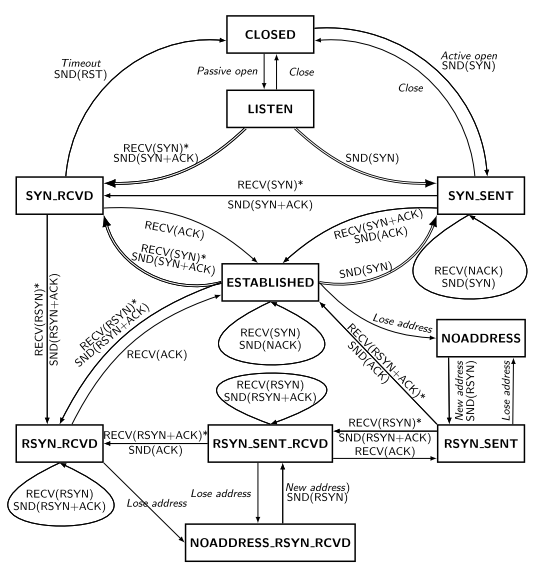
\includegraphics[scale=0.6]{figures/ECCP_sm}
\caption[The ECCP state machine]{The ECCP \cite{Arye2012} state machine.}
\label{fig:EECP_sm}
\end{figure}

This gives the freedom to applications --or even virtual machines-- establish multiple flows, possibly in different interfaces, push and receive traffic to any of them (or a combination of them, increasing bandwidth), without implementing any additional functionality in the protocol residing in the transport layer, or the application.
Everything is settled by the SAL, and a provably correct end-host signalling protocol (figure \ref{fig:EECP_sm}).

When it comes to implementation, flowIDs are 32bit unsigned integers and are end-host specific.
They are created during the synchronization of a new connection and are stored in SAL's flow table, serving as rules for demultiplexing incoming packets to the appropriate sockets.
Source and destination flowIDs are also part of the Serval header in every packet, sitting in the first 64 bits following the IP header.
FlowIDs are persistent throughout the lifecycle of the socket, no matter the modifications of any of the values of the five tuple.


\iffalse
\newpage
\subsection{Service-Level Routing}
\begin{figure}
\centering
\phantomsection
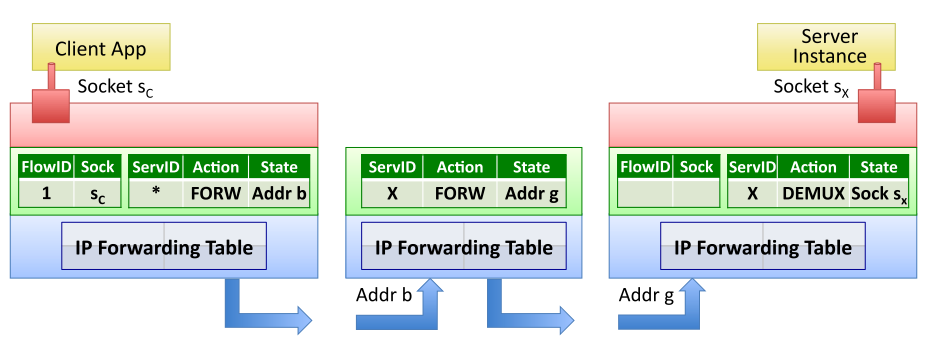
\includegraphics[scale=0.3]{figures/service_level_routing}
\caption[Service-Level Routing]{Service-level Routing based on serviceIDs}
\label{fig:ser_resol}
\end{figure}
No need for deep packet inspection in load balancers
\subsubsection{Late binding}
\fi


\newpage
\subsection{Service name Resolution}
Service names by definition are human readable strings similar to domain names, for identifying services.
Consequently they are in a format that is incompatible to Serval active sockets API.
A method is needed, for mapping those hexadecimal strings to serviceIDs, so they can traverse the network in the service-level routing process described in the previous section.

Serval does not dictate the way service names are resolved to service instances.
In this section we discuss the different approaches in service resolution, a crucial component of any architecture that aims to be adopted in a wide scale.

What we consider important highlighting, is the belief that not always all clients will want to be part of the same service resolution scheme.
In the beginning of the chapter, we discussed the specificities of consumer and peer-to-peer networks.
Based on today's Internet status, it is safe to assume that the hierarchical resolution model with managing authorities could prevail.
But we can be sure that independent, flat resolution services will emerge in a completely separate namespace, over the same or different network wiring.
Still, developers are the ones who will make the final decision on how client applications resolve a service name and reach a service instance, much alike the way it is now.



\subsubsection{Resolution based on a priori knowledge}
Like in the beginning of the Internet, for the moment Serval applications use hardcoded serviceIDs to reach a service.
Violating in a way the service name abstraction, in this transitional stage, serviceIDs are either defined as constants or passed to the program as arguments.
A preordained hashing algorithm and other conventions are used for orchestrating the service registration and resolution, defining in a manner the namespace bounds.

This technique can also be useful in ad hoc (computer-to-computer) networks, when a client needs to reach a service and there are no service resolution services available.
As well as for supporting bootstrapping in other resolution schemes --in the same way as resolv.conf and port 53 are used now, or a list of nodes is pre-fetched in torrent (DHT) applications.


\subsubsection{Hierarchical Resolution}
\label{sec:hierresol}
Much like to the current domain name system domains \nomenclature{URI}{Uniform Resource Locator}, serviceIDs could be managed by an authoritative organization.
This fits well with serviceIDs' potentiality of being allocated as blocks, to organizations and individuals to manage in a longest-prefix match way.

We can imagine a service similar to resolver, mapping a service name to a serviceID.
Lookups will be forwarded recursively to a greater level if they cannot be answered.
Different hierarchical resolution servers might exist and clients should be able to select which one to use by default.
Network administrators might want to setup private service name resolvers, for caching functionality, blocking specific service names (or a block of serviceIDs), or adding new service name to serviceID relations.



\subsubsection{Flat Resolution Schemes}
Another approach suggested by the authors is that serviceIDs get calculated using a hash function on a service prefix and an application-level unique key.
That key, could be content-specific as well.
For example if the application is a web server, prefix bytes indicate that the service is a web server and the key could be a blog name and so on.

Moreover, if the application-level key is omitted, supporting a completely \emph{semantic-free, flat} namespace is also possible.
By semantic-free\cite{Walfisha2004} reference (SFR\nomenclature{SFR}{Semantic Free Reference}) we mean that service identifiers are completely independent from topological, network, or any other characteristic of the service or the provider.

Likewise torrent DHT networks, in order to be able to become a node in the ring, bootstrapping is required with a list of permanent nodes.
Flat resolution schemes, though not suggested for Internet service resolution, they can be useful when it comes to networks without a hierarchical structure, like datacenter and Wide Area networks.



\subsection{Serval Network Stack}
Unlike other next-generation networking proposals, Serval is neither running in the user space, nor is using a translator.
Nevertheless, it does not replace the existing network stack.
Serval is implemented in a kernel module which places itself within an unmodified stack, coexisting with it.
This way developers may choose to use either PF\_INET or PF\_SERVAL, or even both of them in a single application.

In this section we are concentrating on SAL, the Service Access Layer, which offers functionality any
networked service application could use.


\subsubsection{Service Access Layer}

\begin{figure}
\centering
\phantomsection
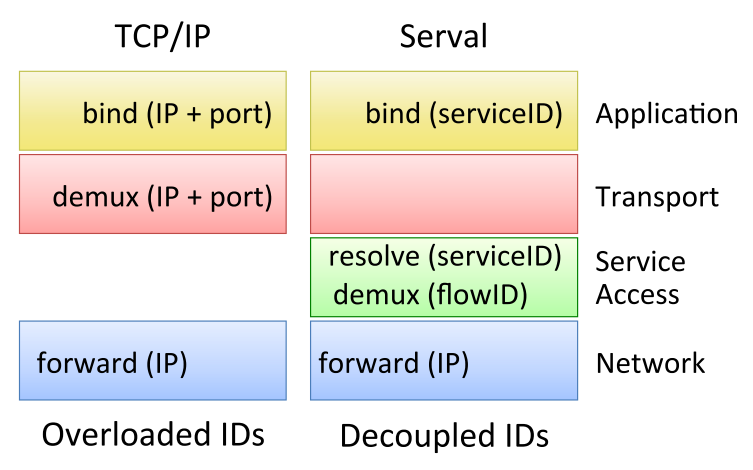
\includegraphics[scale=0.3]{figures/sal_position}
\caption[Service Access Layer position]{Service Access Layer position in the OSI model}
\label{fig:sal_position}
\end{figure}

The Service Access Layer (SAL) is the keystone of the Serval architecture.
Shipped as serval.ko kernel module, SAL bridges the gap between the application layer and the network layer, and undertakes the operations of service resolution, end-to-end signalling, service registration and so on.
Also it provides the hooks for applications to use Serval active sockets.
In fact, all the "magic" behind Serval is implemented in this module, which can be virtually positioned between the Network and the Transport layers in the OSI\nomenclature{OSI}{Open Systems Interconnection model} model (figure \ref{fig:sal_position}).

Extra points go to SAL for being positioned below the transport layer, therefore being transport-protocol agnostic.
This means that developers may choose to use either TCP, UDP\nomenclature{UDP}{User Datagram Protocol}, ATP\nomenclature{ATP}{AppleTalk Transaction Protocol}, FCP\nomenclature{FCP}{Fibre Channel Protocol} or actually any transport protocol, since it is supported by SAL, without modifying the source code of their application.
This opens new windows for experimentation and innovation.

SAL is consisted of two tables, the Service table and the Flow table.
The Service table, the core behind the service-level data plane, contains the rules that correspond to incoming packets with SAL headers and outgoing requests.
The Flow table contains rules for demultiplexing traffic to the appropriate active socket.

\paragraph{Service Table} The Service table contains rules which correspond to one of the following actions:
\begin{enumerate} \itemsep1pt \parskip0pt 
\parsep0pt
  \item \emph{FORWARD}: forwards the packet to the defined IP address.
  That address can also be a multicast, or the IP address of a Service Router. \nomenclature{SV}{Service Router}
  \item \emph{DEMUX}: Demultiplex the packet according to Flow table entries.
  \item \emph{DELAY}: Queue the packet and notify the Service Controller.
  \item \emph{DROP}: Discard the packet.
\end{enumerate}

\paragraph{Flow Table} The flow table 

SAL's position below the transport layer makes it necessary to have a mechanism for decoupling incoming traffic with a DEMUX rule on the service table, to the appropriate socket.
The flow table is responsible exactly for that.
Rules are inserted and removed as soon as there is a change in the flows or the sockets, for example when a socket is closed or when SAL decides to add a new flow to a different interface for an existing socket.
A flow table entry is a simple $<$FlowID, Socket$>$ tuple.




\subsubsection{Serval Packets Structure}
Serval packets are constructed in SAL, using from bottom to top the network layer IP header, Serval header and extensions, and a transport protocol's headers.

Physical, datalink and network layer headers are the common ones one would expect to find.
This is because SAL is not involved in exchanging packets in any level.
Therefore until a packet reaches SAL (service table and flow table), it is processed by middleware as a normal TCP/IP packet in order to reach its final destination.
This feature makes Serval compatible with existing hardware and could assist in its incremental deployment.

In the Service Access Layer level, an extra SAL header is added of minimum 12 bytes.
The structure, is presented in table~\ref{table:salheader}.
\begin{enumerate} \itemsep1pt \parskip0pt 
\parsep0pt
  \item First 4 bytes represent the source flowID of the packet.
  \item The next 4 bytes represent the destination flowID of the packet.
  This is used for demultiplexing with a local socket.
  \item The next byte, marked as SAL Header Length, gives the total SAL header length, including extensions, in 4byte words.
  For a packet that carries payload and no extensions the value is 3.
  \item The 10th byte indicates the protocol of the transport layer which is used; 6 for TCP and 17 for UDP.
  \item The last 2 bytes of the header are used as checksum.
\end{enumerate}

\begin{table}
\begin{center}
  \begin{tabularx}{\linewidth}{|c|X|X|X|X|}
  	\hline
  	Octet &	0 & 1 & 2 & 3 \\ \hline
  	0 & \multicolumn{4}{c|}{Source FlowID}\\ \hline
  	4 & \multicolumn{4}{c|}{Destination FlowID}\\ \hline
  	8 &	Header Length & {Transfer\linebreak Protocol} &	\multicolumn{2}{|c|}{Checksum}	\\
	\hline
  \end{tabularx}
  \caption[Serval packet header structure]{Serval packet header structure}
  \label{table:salheader}
\end{center}
\end{table}

During the initialization of a connection, destination flowID is zero (0).
The next packet though returns both the flowID in the server side and the serviceID once again, to identify which service the response comes from; quite useful for the case of concurrent service resolution requests.

\newpage
When the SAL header length is greater than 3, then there are extensions in the header.
There are 5 types of extensions:
\begin{enumerate} \itemsep1pt \parskip0pt 
\parsep0pt
  \item SAL\_PAD\_EXT
  \item SAL\_CONTROL\_EXT
  \item SAL\_SERVICE\_EXT
  \item SAL\_ADDRESS\_EXT
  \item SAL\_SOURCE\_EXT
\end{enumerate}
In total the extensions included in a packet can not exceed 10.
\\ The SAL\_PAD\_EXT is a special kind of header, of just 1 byte, which helps align the extensions to 8-byte blocks.
\\[0.2cm]
\noindent For easier debugging of Serval packets, we created a LUA Wireshark dissector.
Source code and instructions are attached in the Appendix \ref{sec:wirlua}.



\newpage
\subsection{Service Controller}

\begin{figure}
\centering
\phantomsection
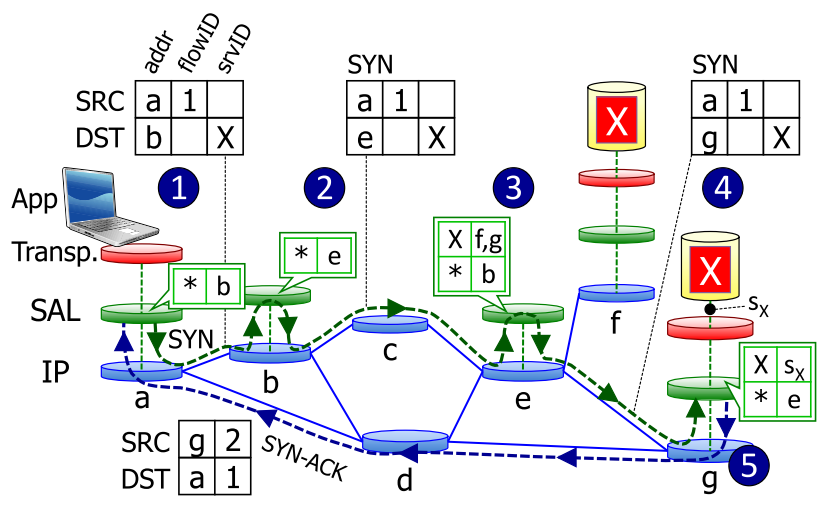
\includegraphics[scale=0.4]{figures/establishing_connection}
\caption[Service Resolution with Service Routers]{Service Resolution with Service Routers}
\label{fig:sal_position}
\end{figure}

Service controller is the key differentiator factor of Serval that elevates services to first-class citizens in the management of the network control plane.
Implemented as a daemon running in the user space, the service controller has direct access to the service table in SAL.
Therefore it can be handy when control-plane logic is needed, as for example in a DELAY action rule in the service table.

Also the Service Controller can out-band communicate with other controllers, distributively deciding the appropriate actions for managing service table entries.
Nevertheless, a network-wide centralized controller could be the one setting service rules in each Serval-enabled node.
This possibility opens new horizons in how next-generation networks could be dynamically configured. 



\subsection{Incremental migration to Serval}
With Serval being actively under development, it is time to discuss the deployment approaches that could guide us to something that has never happened before; the wide adoption of a new network stack.
Above all, benchmarks prove that introducing Serval in large scale networks as well as datacenters offers a wide range of new functionality in speeds comparable to the original TCP/IP stack ones. However, with Internet being a massive diverse network controlled distributively by assorted interest groups --vendors, ISPs, service providers--, deployment of a new networking architecture is a real nightmare \cite{Podmayersky2011}.
\\ \indent Prime example is the adoption of IPv6. Intending to solve the problem of IPv4 exhaustion, IPv6 uses 128-bit addresses (in comparison to IPv4's 32-bit IP addresses), providing approximately 4.3 billion addresses for network interfaces. Still, after over a decade of protracted efforts, less than 4\% \footnote{Visualization based on original data from RIR, routeviews, Alexa, Google, ITU and APnic by Cisco at \url{http://6lab.cisco.com/stats/}} of Internet global traffic is carried over it, although it is a necessary to take step for the next generation of the Internet of Things. \nomenclature{IoT}{Internet of Things}
\\ \indent A smooth transition to a new architecture requires two things: first that current hardware and intermediary devices are compatible or at least do not interfere with the new packet headers, and that applications are utilizing the late interfaces and are able to dissect and synthesize those packets.

\subsubsection{Legacy Hardware}
SAL's position just on top of the network layer makes it translucent to networking equipment such as hubs, switches and routers, since they are messing up with the headers of up to the network layer.
At this level, hardware is responsible only for delivering the packets to the right destination, the way they have been doing so far.
\\ \indent Serval on the contrary is not immune to stateful packet inspection\nomenclature{SPI}{Stateful Packet Inspection} and deep packet inspection\nomenclature{DPI}{Deep Packet Inspection}.
Intermediaries who access the headers of the transport or above layers will have a hard time dissecting a minimum 32 extra bytes following the network layer.
The use of NAT-based\nomenclature{NAT}{Network Address Translator} agents though, such as load balancers, can be obscured due to the late binding on serviceIDs.
In any way, operation behind legacy networks middleware can be achieved via UDP encapsulation.
\\ \indent Apparently, even if typical routers are compatible with routing Serval packets, they cannot provide service-level routing, service registration, unregistration and propagation, or any other feature of a Serval router\footnote{The generation of routers that supports virtual services, such as the Cisco Nexus series 1100, might be able to imitate features of a service router with a virtual service.}.
Hopefully this is not a blocking obstacle, as far as the SAL knows a service router that can forward service name resolution requests to.
That service router might be deep within the network and not accessible through service propagation.

\subsubsection{Modified Programming Interfaces}
Unlike other proposals which can be either integrated in programs as libraries or provide abstractions by overloading identifiers such as ports, Serval's kernel module implementation requires applications to be modified in order to use its active sockets API.
\\ \indent In other words, a minimum port of an existing applications would require to include and link to \textless libserval/serval.h\textgreater ~and \textless netinet/serval.h\textgreater ~libraries, set socket family to AF\_SERVAL and substitute system calls to the socket layer such as connect, bind, accept, send etc to use serviceIDs.
Minor modifications might be needed, since new identifiers require different size of bytes to be allocated in memory and so on.
\\ \indent The complexity of porting an existing application to Serval depends on how neatly is the connection module isolated.
In general, applications that support various protocols are easier to be ported, since connectivity functions are already decoupled from the program logic and can be replicated to support new APIs.
Large applications, with thousands lines of code,\nomenclature{loc}{lines of code} like Mozilla Firefox require modifications in around just 70 lines of code.
Design patterns like singleton and factory noticeably indicate which parts of the source code should be altered.
\\ \indent Nevertheless, applications can simultaneously support multiple protocols and stacks, according to the requests of the other end.
This will be a great advantage in the transitory period of large scale deployment.
\\ \indent On the other hand, unexpected runtime results might be confronted due to overlapping of features offered by SAL and reimplemented in the program.
For instance service load balancing at SAL, an inherent component of Serval, might muddle with the application-specific way of allotting requests.
In such cases if possible one of the methods should dominate the final decision.
Either a unique serviceID of an allocated serviceID block --as described in the Hierarchical Resolution approach-- should be used for each instance, and let load-balancing be made by application's functions.
Or load-balancing logic within the application should be removed when a socket's family is AF\_SERVAL and be managed according to service-level rules defined in SAL.
\\ \indent As a reference you can find a diff file from the port of nginx\footnote{Nginx [engine-ex] is an Open Source HTTP, reverse proxy and mail proxy server\\ \url{http://nginx.org/}.} to Serval in the appendix \ref{sec:nginxport}.
This diff version includes the integration of the [nginx\_1.2.9\_serval\_fqdn] branch commits from \mbox{sns/Serval} repository into the build procedure.

\subsubsection{Incremental Deployment with Serval translator}
\begin{figure}
\centering
\captionsetup{justification=centering}
\phantomsection
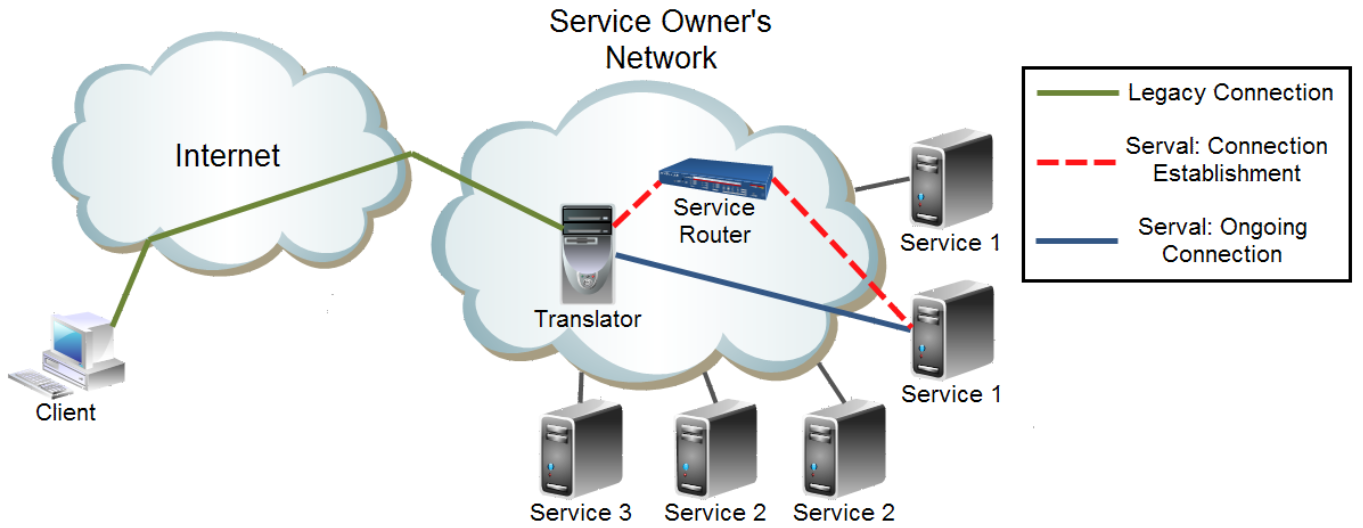
\includegraphics[scale=0.25]{figures/Serval_translator}
\caption[Serval translator]{A Serval translator as an intermediary\\for communicating with legacy clients \cite{Podmayersky2011}.}
\label{fig:serval_translator}
\end{figure}
The Internet has expanded in a level where migrating to a new architecture through a coordinated "flag day", where we disconnect all devices in order to cold-plug update them, is an unnegoatiable scenario.
Downtime, unreachable hosts running on embedded hardware, telecommunications, are only a few of the reasons that induce a gradual strategy when it comes to adopting Serval.
\\ \indent As observed in similar examples, the ones expected to make the first move are service providers.
Both for the reason that they are greatly benefited by this migration, as well for their pertinent awareness.
In order to face the challenge of serving both legacy and Serval-enabled clients, Brandon Podmayersky implements a \emph{Serval translator} \cite{Podmayersky2011}, an intermediary service which can be hosted in a middlebox machine or on the server itself, and which bridges the connection between a service using Serval active sockets and legacy TCP/IP clients.
\\ \indent Serval translator works on the simple principle of exposing legacy TCP/IP interfaces to the outer network --may it be the Internet--, which are then translated to Serval active sockets.
The procedure is illustrated in Figure~\ref{fig:serval_translator}.
Legacy clients resolving a service name via a search mechanism, may it be DNS, get the public-facing IP address of the translator in front of the corresponding service.
Then they are connecting with that IP and a well-known port directly to the Serval translator, opening a typical AF\_INET socket.
The predefined port as anyone would expect can be the default legacy port of the service the client wants to reach (for a web server that would be port 80).
Note that a translator might be the first point of contact for multiple services, with its IP address registered --similar to a DNS A record-- for various service names and mapping requests to different ports to different services or service instances.
This mapping actually links an $<IP, port>$ tuple to a serviceID, which then can be resolved using the service table of SAL, or custom load balancing rules. 
After that, the translator takes care of the connection synchronization with the service, and splices\footnote{splice() is a system call introduced in the 2.6.17 kernel, that can move data between two file descriptors without copying between kernel address space and user address space\\ \url{http://linux.die.net/man/2/splice}.}
When the connection is terminated, the translator closes the sockets at both ends.
\\ \indent Using the Serval translator a service provider can handle requests from both legacy and Serval-ready clients.
Requests that have a serviceID get routed directly to the service instance, overpassing the translator.
However, on an established legacy connection, every single packet is processed by the translator, modifying headers and flags appropriately.
This indeed adds an overhead and indicates a possible single point of failure, but benchmarks show its performance is good enough to be deployed in real networks and a cluster of such translators can be used in a hierarchical schema.
\newpage
\subsection{Profiling the Serval prototype implementation}
Among the admirable headliners of Serval is the working prototype version of the proposed architecture.
In more than 28000 lines of code\footnote{Serval is an Open Source project, hosted at a public repository\\ \url{https://github.com/princeton-sns/serval/}.} covering functionality of the Service Access Layer (both in userlevel operation and as a Linux kernel module), bindings for multiple programming languages, a translator, libraries and examples for writing Serval compatible applications, and with a reported throughput comparable to the unmodified TCP/IP stack, it is clearly showcased the feasibility of the solution.

In this section we are profiling the prototype in regard to the following parameters:
\begin{enumerate} \itemsep1pt \parskip0pt 
\parsep0pt
  \item CPU Instructions and Cycles
  \item System Call execution times
  \item Execution time needed for the completion of a numbered iteration of requests
  \item Number of packers per request, bytes on the wire
\end{enumerate}
Then we will be presenting the results juxtaposed to the measurements of the unchanged TCP/IP stack and the AF\_INET family.

\paragraph{} Output was obtained on a HP Prodesk 600 G1 --Intel(R) Core(TM) i5-4570 @ 3.20GHZ, 4GB RAM-- machine running Ubuntu 11.04 (Natty Narwahl) kernel version 2.6.38-16-generic (rebuilt with debug symbols).

The profiling tools we used include gprof, perf, oprofile, valgrind, strace, zoom and google performance tools.
For the tests with gprof, valgrind, oprofile and strace, Serval module and http\_client were built with debug symbols.
Extra, for gprof testing, Serval was built with CFLAGS, LDFLAGS and CPPFLAGS equal to "-pg".

For the measurements we ported libmicrohttpd to use Serval active sockets.
Also, we implemented a simple HTTP client which supports both AF\_INET and the AF\_SERVAL socket families, depending on the options passed during the call.
For each case, we used the INET and Serval version of librehttpd and http\_client respectively.
Therefore, besides the connectivity parts, both INET and SERVAL versions are working with the same logic in creating, exchanging and processing requests.
This way we believe the tests can give unbiased results, which would not be the case if for example we used Apache server for INET and libmicrohttpd for SERVAL requests.

Source code of libmicrohttpd and http\_client, along with the integration of Serval patch in the build procedure of nginx, can be found in the Appendix (\ref{sec:appendix}).
Benchmark results are published in the ServalDHT repository \footnote{\url{https://github.com/misaakidis/ServalDHT}}.



\subsubsection{Serval's performance in the worst case scenario}
In a network architecture benchmarking what matters the most is its total throughput under a stress test.
In other words, the data rate of information (both headers and payload) and the number of packets that can be processed during a specific time frame.
An excellent tool for this case, \emph{iperf}, proved Serval's TCP throughput to be very close to the original TCP's one, almost fully utilizing a GigE interface. \nomenclature{GigE}{Gigabit Ethernet}
The authors explain that the existing small difference is due to missing optimizations in Serval's prototype.

We are examining Serval from a completely different perspective.
We dive into the implementation of SAL and serval.ko module and the overhead in using the Serval APIs.
And we do so in the worst possible scenario for an architecture that is establishing its own identifiers in the end host stacks.

It is SAL's responsibility to create the flows and synchronize the sockets in either side \footnote{Specifically for TCP, Serval is using the functionality that corresponds only to the ESTABLISHED state.}.
This means that when binding an active socket to a serviceID, the SAL must insert an entry into the flow table, register the service in the service table with a DEMUX rule and propagate the service registration to the network (may it be an anycast flood or a request to a singe service router).
Also, when connecting to a service, SAL must first convert a service name to a serviceID, resolve the serviceID, and finally establish a connection using CONTROL and SERVICE headers.
Correspondingly, closing a connection requires the exchange of packets with CONTROL headers.
In both cases, must-have checks like whether a serviceID is of an appropriate format, are more computational effort to the perquisite ones.

Once a connection has been established, the only significant overhead is the addition of a 12 bytes Serval header with the source and destination flowIDs, and the demultiplexing of incoming packets.
We can presume for those reasons, that Serval (and any other relative architecture) is struggling during the process of establishing a connection.

The case scenario we are testing is consisted of a client that connects to a service and requests information that can fit within a single response packet.
Since both the server and the client are running in the same machine, we can presume that the available bandwidth exempts network "links" from being responsible for a bottleneck.
The results show how well the Serval implementation can manage when it is pushed to the limit.



\newpage
\paragraph{Instructions and CPU Cycles} \hfill \\
Using perf performance counters subsystem in Linux \footnote{\url{https://perf.wiki.kernel.org/}}, we were able to benchmark the http\_client application with PF\_INET and PF\_SERVAL socket protocol families in a CPU cycle level.
There is definitely an increase in the Instructions and CPU cycles of the PF\_SERVAL version, as presented in Table \ref{table:cpu}, but taking a closer look in the perf output one will notice that there is a great increase in cache-misses and in the amount of branches.
Therefore the Instructions increase is a less biased index of the complexity added in the Serval port.
\begin{table}
\begin{center}
  \begin{tabular}{l||cc|cc|c}
  	\toprule
  	Metric			&	\multicolumn{2}{c}{PF\_INET}	&	\multicolumn{2}{c}{PF\_SERVAL}	&	Increase	\\
  	\midrule
    Instructions	&	690,559		&	$\pm$0.009\%	&	1,864,287	&	$\pm$0.054\%	&	169.9\%		\\
    CPU Cycles		&	1,019,096	&	$\pm$0.062\%	&	8,799,912	&	$\pm$0.191\%	&	763.5\%		\\
    Cache-misses	&	685			&	$\pm$1.417\%	&	72,893		&	$\pm$0.217\%	&	10541.3\%		\\
    Branches		&	125,548		&	$\pm$0.009\%	&	348,329		&	$\pm$0.057\%	&	177.4\%		\\
    \bottomrule
  \end{tabular}
  \caption[Benchmark: Instructions and CPU Cycles]{Instructions and CPU Cycles in 10000 runs of http\_client}
  \label{table:cpu}
\end{center}
\end{table}



\paragraph{System Calls execution times} \hfill \\
The results in Table \ref{table:stat} from stat user call \footnote{\url{http://man7.org/linux/man-pages/man1/stat.1.html}} show the independence of the time system calls need to complete, regardless the use of INET or SERVAL protocol family sockets.
This was expected and validated, since SAL in the kernel level is using the same system calls for its networking functions.
\textbf{\begin{table}
\begin{center}
  \begin{tabular}{l||c|c}
  	\toprule
  	Syscall			&	PF\_INET	&	PF\_SERVAL	\\
  	\midrule
    socket			&	0.145		&	0.070		\\
    setsockopt		&	0.160		&	0.118		\\
    connect			&	0.117		&	0.113		\\
    getsockname		&	0.300		&	0.552		\\
    send			&	0.089		&	0.086		\\
    recv			&	0.159		&	0.313		\\
    close			&	0.086		&	0.087		\\
    \bottomrule
  \end{tabular}
  \caption[Benchmark: System Call execution times]{Kernel System Calls execution times (in milliseconds)}
  \label{table:stat}
\end{center}
\end{table}}



\newpage
\paragraph{Finite Requests loop timing} \hfill \\
In this test we calculate --again using perf-- the milliseconds needed for the execution of a single request.
It is noteworthy that after a number of requests the execution time fails significantly.
Results listed in Table \ref{table:reqtime}
\begin{table}
\begin{center}
  \begin{tabular}{l||cc|cc|c}
  	\toprule
  	Requests	&	\multicolumn{2}{c}{PF\_INET}	&	\multicolumn{2}{c}{PF\_SERVAL}	&	Increase	\\
  	\midrule
    10			&	1.171		&	$\pm$2.171\%	&	1.845		&	$\pm$1.542\%	&	57.5\%		\\
    100			&	0.399		&	$\pm$7.248\%	&	0.686		&	$\pm$9.404\%	&	71.9\%		\\
    1000		&	0.590		&	$\pm$5.835\%	&	0.837		&	$\pm$7.751\%	&	41.9\%		\\
    \bottomrule
  \end{tabular}
  \caption[Benchmark: Requests execution times]{Requests execution times}
  \label{table:reqtime}
\end{center}
\end{table}



\paragraph{Packets specific metrics} \hfill \\
After all, we are focusing on the packets sent for each HTTP request.
Serval again has to send 5 more packets with control headers for the establishment and closing of the connection.
Finally there is an increase in the bytes transferred on the wire.
It is wise to highlight at this point that in a case where the payload would need to be split in more packets, or the conenction to be used as a stream for communication, that the observed overhead of extra packets would be negligible, and only the 12-byte header of serval would add bits on the stream.
\begin{table}
\begin{center}
  \begin{tabular}{l||c|c}
  	\toprule
  	Metric				&	PF\_INET	&	PF\_SERVAL	\\
  	\midrule
    Packets/request		&	10			&	15			\\
    Bytes/request		&	922			&	1392		\\
    \bottomrule
  \end{tabular}
  \caption[Benchmark: Packets and bytes exchanged per request]{Packets and bytes exchanged per request}
  \label{table:packets}
\end{center}
\end{table}



\newpage
\subsubsection{Benchmark results files}
As a reference, you can find the results of performance testing in the public repository, under the \emph{benchmarking} directory.
Specifically for INET and SERVAL you will find:
\begin{enumerate}
  \item \emph{gprof\_httpclient}: Results from gprof profiling tool. One can see the call graph of http\_client. Execution is completed fast enough to show zero accumulated time with the 0.01 seconds samples.
  \item \emph{kcachegrindgui\_httpclient}: Annotated source code with valgrind's kcachegrind tool.
  \item \emph{kcachegrind\_httpclient}: Graphic representation of the call tree along with the Instructions of each function.
  \item \emph{libmicrohttpd\_wireshark.pcap}: Wireshark capture of INET and SERVAL sockets with the libmicrohttpd server.
  \item \emph{nginx\_wireshark.pcap}: Wireshark capture of INET and SERVAL sockets with the nginx server.
  \item \emph{opannotate\_httpclient}: Percentage of time spent on each file called (including shared libraries). Vmlinux corresponds to kernel space processes.
  \item \emph{perf\_httpclient}: Performance counter stats 10,000 requests.
  \item \emph{perf\_serval\_mod}: Map details of the serval dynamically shared object (dso). DSOs are the "gateway" between the user and kernel space, and act as the contact point when an application running in the user space makes a system call.
  \nomenclature{DSO}{Dynamically Shared Object}
  \item \emph{statc\_httpclient}: List of system calls.
  \item \emph{stat\_httpclient}: Ordered system calls with their execution time.
\end{enumerate}



\newpage
\subsubsection{Closing remarks on benchmark results}
Results from performance testing might be alerting.
As closing remarks of the benchmarking section, we would like to shape our thoughts on the topic.

Serval is a great, well-thought service-centric network architecture.
Its simple, genuine abstractions, its clean separation of the control and the data plane, its resilience in migration, its familiar APIs, all add upon a networking model which provides apparent benefits to service providers and users as well.

However, services have some congenital characteristics that are not met on all networked applications.
Above all, services rely on resolute connections.
Once the path is established, a flow is expected to retain its reachability and serve as the channel for constant communication with the other side.
A channel which ordinarily serves as the middle for large files exchange.
Thereupon, SYN packets are only a small proportion of the network traffic of services.
A small overhead thus in the connection establishment is acceptable, especially if it can prevent a future reinitiation of the same process.

In contrast, there are applications which are working in a completely different way.
Programs that wake up one in a day to send a single packet to a remote server.
Real time systems that have to deliver a small part of information to many recipients.
Embedded machines that produce burst data and which do not require every single packet to be delivered.

Those scenarios are far from rare.
VoIP, \nomenclature{VoIP}{Voice over IP} media streaming, online games, even the DNS itself are illustrative examples.
For many years now we have been treating them in a special way; connectionless communication.
UDP over TCP has been serving well in those situations that we want to send fast, limited amount of data or when we do not care about if the packets get delivered.

We understand that the tests conducted do not represent a common use case.
They indicate though a possible shortcoming of Serval and demonstrate an expected performance in the worst scenarios as described above.

In the long run, Serval should not be considered a nostrum.
As every networking paradigm, it servers best where it was originally intentioned to do so.
SAL's symbiotic capability with the TCP/IP stack gives us the final choice to reason in which circumstances to use the Serval APIs and when to follow the well-trodden path.


%%%%%%%%%%%%%%%%%%%%%%%%%%%%%%%%%%%%%%%%%%%%%%%%%%%%%%%%%%%%%%%%%%%%
\newpage
\thispagestyle{empty}
\phantomsection
\addcontentsline{toc}{part}{Relative Bibliography}
{\Huge \bf \noindent RELATIVE BIBLIOGRAPHY}
\newpage

\section{Review of relative bibliography}
ServalDHT is a multifaceted architecture that combines ideas from a wide spectrum of topics, including but no limited to Large Scale Network Architectures, Network Protocol Layers, Service-Centric Networking, Software Defined Networking, Distributed Hash Table algorithms and security issues of their various implementations, Peer-To-Peer Lookup Services as a replacement to legacy DNS etc.
Therefore references should contain an adequate number of publications on all those themes.\\
\indent The publications that have been used so far as a source of information follow in section 7.
Brief summaries can be found in Appendix at the end of the report.


\subsection{Decoupling a Host Identity from its location}
\subsubsection{HIP}
\subsubsection{DOA}
\subsubsection{LISP}
\subsubsection{LNA}
\subsubsection{HAIR}
\subsubsection{i3}


%%%%%%%%%%%%%%%%%%%%%%%%%%%%%%%%%%%%%%%%%%%%%%%%%%%%%%%%%%%%%%%%%%%%
\newpage
\thispagestyle{empty}
\phantomsection
\addcontentsline{toc}{part}{Rethinking Networking}
{\Huge \bf \noindent RETHINKING NETWORKING}
\newpage

\section{Rethinking the Internet experience}
%I HAVE A DREAM
Cloud computing
\\Modularity
\\anonymity, privacy
\\authentication, accountability, encryption, security
\\no middlewares
\\TCP/IP stack data, controller functionality
\\subnetworks
\\mobility and multihoming
\\independent from organizations


%%%%%%%%%%%%%%%%%%%%%%%%%%%%%%%%%%%%%%%%%%%%%%%%%%%%%%%%%%%%%%%%%%%%
\newpage
\section{Service-centric architectures and SDN}
A well thought Service centric architecture provides two things
the right abstractions for services (developers and users)
a service-aware control plane

So that control plane could be merged with software defined networking apis
sdn apis that have control over the fabric of the network

as a result: sal can manipulate the virtual network
dynamic policy-driven networking
split control (sal AND sdn controller decide)
distributed management
immediate effect
larger scale service-level routing



\subsection{Scenario: Service Registration as a Network Policy}
Scenario:
service registration as policy


%%%%%%%%%%%%%%%%%%%%%%%%%%%%%%%%%%%%%%%%%%%%%%%%%%%%%%%%%%%%%%%%%%%%
\newpage
\section{Service-Aware Networking and Cloud Networks}
How can we take advantage of the above mentioned results in cloud networks?
why cloud fits the description


%%%%%%%%%%%%%%%%%%%%%%%%%%%%%%%%%%%%%%%%%%%%%%%%%%%%%%%%%%%%%%%%%%%%
\newpage
\section{Introduction to the Proposed Solution}
User Serval as it is, but with a Distributed Service Resolution Service
\\Based on DHT algorithms
\\Run by tier-1 and ISPs, or by users in Autonomous networks
\\Secure identifiers
\\Flat namespace
\\Gets serviceID and
\\- either returns the (IP,Port) back to the client
\\- or forwards the packet directly to the service provider
\\- caches the (serviceID, IP) tuple for future use
\\Incrementally deployable and backwards compatible
\\written in C, running in the user space
\\accept service registration, checks HIP and inform the relative nodes
\\About the Service Controller:
\\will be running as a daemon in the userspace
\\will communicate with ServalDHT to resolve serviceIDs (hashed service names)
\\will enable delegation, load balancing etc as modules (maybe a configuration file?)
\\Draw a FSM for the SRS \nomenclature{SRS}{Service Resolution Service} (http://madebyevan.com/fsm/)


%%%%%%%%%%%%%%%%%%%%%%%%%%%%%%%%%%%%%%%%%%%%%%%%%%%%%%%%%%%%%%%%%%%%
\newpage
\section{Future Research}
1. Implement Service Controller (compatible with OpenFlow)
\\2. Implement ServalDHT SRS
\\3. Results of deployment in PlanetLab
\\4. Start preparing an RFC?
\\See how DHTs can replace hierarchical DNS?


%%%%%%%%%%%%%%%%%%%%%%%%%%%%%%%%%%%%%%%%%%%%%%%%%%%%%%%%%%%%%%%%%%%%
\newpage
\phantomsection
\addcontentsline{toc}{part}{Bibliography}
{\Huge \bf \noindent Bibliography}
\nocite{*}
\bibliographystyle{plain}
\renewcommand{\refname}{}
\bibliography{bibliography}


%%%%%%%%%%%%%%%%%%%%%%%%%%%%%%%%%%%%%%%%%%%%%%%%%%%%%%%%%%%%%%%%%%%%
\newpage
\pagestyle{empty}
{\Huge \bf \noindent APPENDIX}
\phantomsection
\addcontentsline{toc}{part}{APPENDIX}
\newpage

%%%%%%%%%%%%%%%%%%%%%%%%%%%%%%%%%%%%%%%%%%%%%%%%%%%%%%%%%%%%%%%%%%%%
\newpage
{\Huge \bf \noindent A. PRESENTATIONS}
\phantomsection
\addcontentsline{toc}{section}{A. Presentation}

\newpage
\phantomsection
{\huge \bf \noindent A.1 ServalDHT - Secure DHT\\[0.2cm] based Service Resolution Service}
\label{sec:servaldhtpres}
\addcontentsline{toc}{subsubsection}{A.1 ServalDHT - Secure DHT based Service Resolution Service}
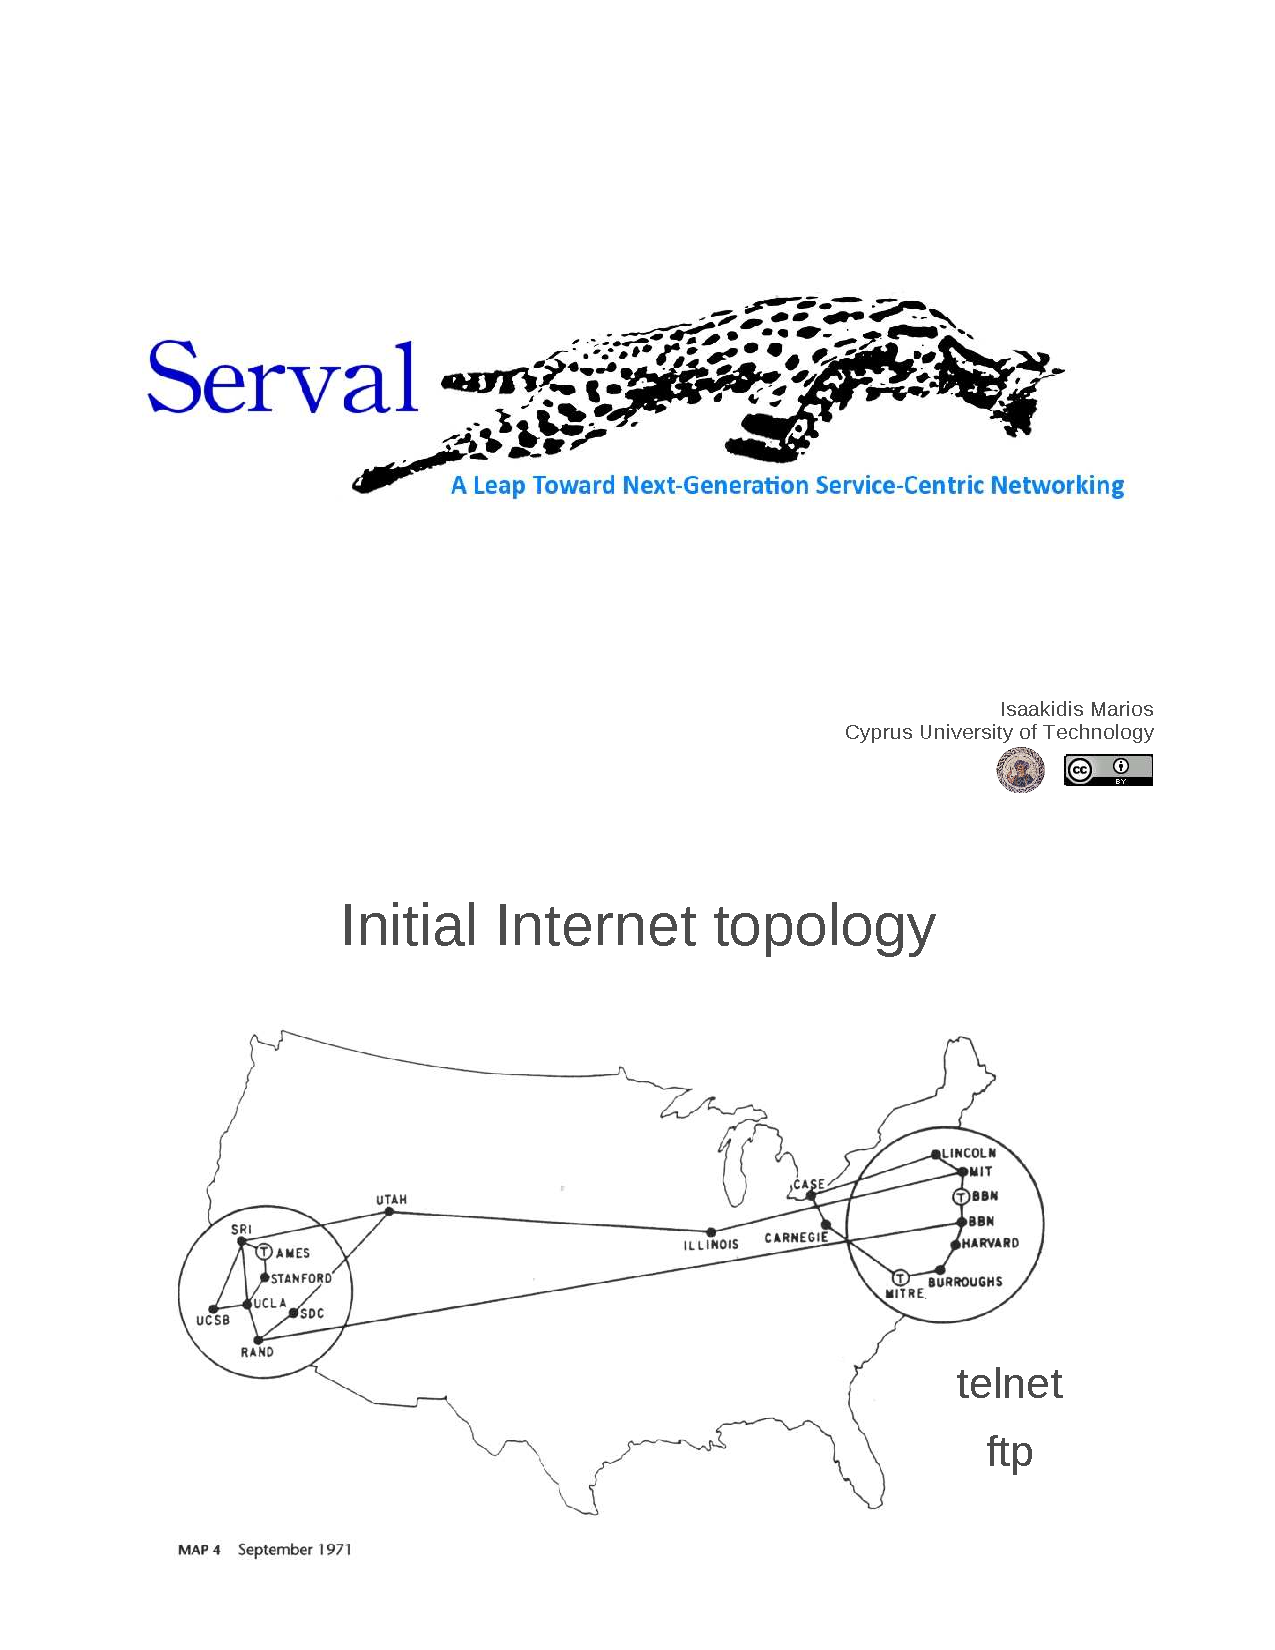
\includepdf[pages={-}]{ServalDHT-Pres2.pdf}


%%%%%%%%%%%%%%%%%%%%%%%%%%%%%%%%%%%%%%%%%%%%%%%%%%%%%%%%%%%%%%%%%%%%
\newpage
{\Huge \bf \noindent B. SOURCE CODE}
\phantomsection
\addcontentsline{toc}{section}{B. Source Code}
\label{sec:sourcecode}


%%%%%%%%%%%%%%%%%%%%%%%%%%%%%%%%%%%%%%%%%%%%%%%%%%%%%%%%%%%%%%%%%%%%
\newpage
{\huge \bf \noindent B.1 nginx serval port}
\addcontentsline{toc}{subsubsection}{B.1 nginx serval port}\\[0.5cm]
\textbf{File:} ports/nginx/nginx-1.2.9-integrated-serval.patch\\
\textbf{Description:} Patch nginx version 1.2.9 to use Serval active sockets. \\
\textbf{Instructions: }
\begin{enumerate} \itemsep1pt \parskip0pt 
\parsep0pt
	\item Apply the patch using git
	\item Copy libraries from serval/include to a path included in the search path of your compiler (normally that should be /usr/local/include/)
	\item Configure nginx with serval (ports/nginx/configure --with-serval)
	\item Make sure configure script found netinet/serval.h library and can build AF\_SERVAL
	\item If everything is fine, you should be able to see "+ using serval active sockets" in the configuration summary
	\item Compile with make and then execute make install
	\item Edit nginx configuration file (by default /usr/local/nginx/conf/nginx.conf) and uncomment the virtual host configured for the serval architecture
	\item Restart nginx and now you can accept both AF\_INET and AF\_SERVAL requests
	\item nginx Service ID is 8\\[0.5cm]
\end{enumerate}
\lstinputlisting[language=diff]{source_code/nginx-1.2.9-integrated-serval.patch}



\end{document}